%=========================================================================
% sec-intro
%=========================================================================

\section{Introduction}
\label{sec-intro}

\begin{figure}[b]
  \begin{minipage}[b]{0.42\tw}
    %=========================================================================
% fig-intro-overview
%=========================================================================

%\begin{figure}

  \centering
  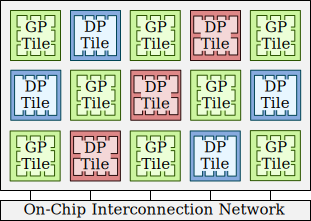
\includegraphics[width=\tw]{intro-overview.svg.pdf}

  \caption{\textbf{Example of Fine-Grain Heterogeneous Architectures --}
    A sea of lightweight compute tiles composed of both general-purpose
    tiles (CPUs) and accelerators specialized for exploiting varying
    forms of parallelism (GPUs for graphics and DSPs for digital signal
    processing).}

  \label{fig-intro-overview}

%\end{figure}

  \end{minipage}%
  \hfill%
  \begin{minipage}[b]{0.56\tw}
    %=========================================================================
% fig-intro-vision
%=========================================================================

%\begin{figure}

  \centering
  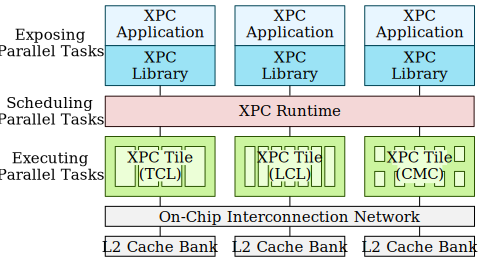
\includegraphics[width=\tw]{intro-vision.svg.pdf}

  \caption{\textbf{XPC Architecture Overview --} XPC applications use an
    XPC parallel programming library to expose fine-grain parallel
    tasks. A software runtime is used to facilitate adaptive task
    distribution to the available hardware resources based on collected
    heuristics. Heterogeneous XPC tiles are specialized for various forms
    of parallelism, but all XPC tiles have the same ISA.}

  \label{fig-intro-vision}

%\end{figure}

  \end{minipage}
\end{figure}

Microprocessor design has reached a point where the efficacy of simply
adding more cores onto the chip has been saturated. Due to this and many
other technological challenges, computer architects are increasingly
turning toward new abstractions to take advantage of the growing
transistor density. For example, almost all general-purpose multicores include
limited support for exploiting data parallelism with subword-SIMD
extensions (e.g., Intel SSE~\cite{intel-sse4-manual2007}, IBM Cell SIMD
extensions~\cite{gschwind-ibm-cell-ieeemicro2006}, and
others~\cite{slingerland-simd-survey-ucbtr2000}). A common trend is a
coarse-grain approach to heterogeneous architectures such as Intel
Haswell~\cite{hammarlund-intel-haswell-ieeemicro2014}, AMD
Kabini~\cite{bouvier-amd-kabini-ieeemicro2014}, and NVIDIA Tegra
4~\cite{krewell-nvidia-tegra4-mpr2013}, where general-purpose multicores
are colocated with graphics processing units.

However, emerging trends in applications are demanding a more fundamental
paradigm shift in computer architecture. For example, a ubiquitous type
of \emph{amorphous data parallelism} that encapsulates many types of existing
data parallelism can dynamically modify the underlying data structure as
well as generate most of its work
dynamically~\cite{pingali-tao-pldi2011}. These emerging applications can
be highly unpredictable and also exhibit varying levels of parallelism
based on the phase of execution or input dataset.
%Examples include graph processing, physical simulation, big data
%analytics, large-scale optimization, and machine learning.
GPU vendors are beginning to adopt parallel programming frameworks that
offer limited support for handling amorphous data parallelism at a coarse
granularity and heavily relying on software (e.g., AMD heterogeneous
system architecture~\cite{amd-hsa-wpaper2012} and NVIDIA dynamic
parallelism
constructs~\cite{nvidia-dynamic-parallelism-wpaper2012}). Unfortunately,
the current abstractions for computer architecture are not ideal for the
rapid, dynamic task distribution necessary to fully capitalize on
opportunities for accelerating these emerging applications, largely due
to the complexity of the compute tiles and the cost of spawning parallel
tasks.

In order to address these challenges, this proposal outlines the
Explicit-Parallel-Call (XPC) architecture, a fine-grain heterogeneous
architecture that enables seamless adaptive execution of fine-grain
parallel tasks across a sea of lightweight heterogeneous compute tiles
like shown in Figure~\ref{fig-intro-overview}. It is imperative that a
vertically integrated methodology is used to innovate across the
software/hardware interface in order to address heterogeneous system
complexity and meet the needs of emerging amorphous data parallel
applications. To this end, the vision for the XPC architecture is to
explore both software and hardware techniques for \emph{exposing},
\emph{scheduling}, and \emph{executing} fine-grain parallel tasks as
illustrated in Figure~\ref{fig-intro-vision}.
